\documentclass[sigconf,review]{acmart}
\acmConference[508 UBC]{Operating Systems 508}{Sept-Dec, 2017}{AndyLand UBC}

%\usepackage{times}
%\usepackage{fullpage}
%\usepackage{booktabs}  % for \midrule
%\usepackage{subfigure}
\usepackage{balance}
\usepackage{graphicx}
\usepackage{xspace}
%\usepackage{pslatex}
%\usepackage{pifont}
%\usepackage{multirow}

\usepackage{array}
\newcolumntype{L}[1]{>{\raggedright\let\newline\\\arraybackslash\hspace{0pt}}m{#1}}
\newcolumntype{C}[1]{>{\centering\let\newline\\\arraybackslash\hspace{0pt}}m{#1}}
\newcolumntype{R}[1]{>{\raggedleft\let\newline\\\arraybackslash\hspace{0pt}}m{#1}}


%\usepackage{booktabs}
%\usepackage{cite}
\usepackage{url}
%\usepackage{cancel}
\usepackage{color,colortbl}
%\usepackage{microtype}
%\usepackage{textcomp}% http://ctan.org/pkg/textcomp
%\usepackage{tabularx}
%\usepackage{framed}
\usepackage[]{algorithm2e}
\SetAlFnt{\small}
\SetAlCapFnt{\small}
%\usepackage{algorithmic}

\usepackage{ctable} % for \specialrule command

\usepackage{listings}
%\usepackage{scrextend}
%\usepackage{mathtools}
\usepackage{pbox}

\let\labelindent\relax
\usepackage{enumitem}

%\usepackage[labelfont=bf]{caption}

% Copyright
%\setcopyright{acmcopyright}

%\setcopyright{acmlicensed}
\setcopyright{none}

%\setcopyright{rightsretained}
%\setcopyright{usgov}
%\setcopyright{usgovmixed}
%\setcopyright{cagov}
%\setcopyright{cagovmixed}

\usepackage{listings}
\lstdefinelanguage{cs}
{
  morekeywords={abstract,event,new,struct,as,explicit,null,switch
		base,extern,this,bool,false,operator,throw,
		break,finally,out,true,byte,fixed,override,try,
		case,float,params,typeof,catch,for,private,uint,
		char,foreach,protected,ulong,checked,goto,public,unchecked,
		class,if,readonly,unsafe,const,implicit,ref,ushort,
		continue,in,return,using,decimal,int,sbyte,virtual,
		default,interface,sealed,volatile,delegate,internal,short,void,
		do,is,sizeof,while,double,lock,stackalloc,
		else,long,static,enum,namespace,string,
		where, from, select, group,by, having, into, many,
		every,
                function,
		or, and, on, var, when,let, zip, combine,
		minute,hour,day,week,year,calendar,count, Delay, Until, TakeUntil, Sample, Skip, Throttle},
	  sensitive=true,
	  morecomment=[l]{//},
	  morecomment=[s]{/*}{*/},
	  morestring=[b]",
}

\lstset{
	language=cs,
	tabsize=2,
        basicstyle=\small,
%        basicstyle=\normalsize,
        %upquote=true,
%        aboveskip={1.5\baselineskip},
        columns=fullflexible, %fixed,
        showstringspaces=false,
        extendedchars=true,
        breaklines=true,
%      prebreak = \raisebox{0ex}[0ex][0ex]{\ensuremath{\hookleftarrow}},
%	frame=single,
        showtabs=false,
        showspaces=false,
       identifierstyle=\ttfamily,
        keywordstyle=\color[rgb]{0,0,.8},% \sffamily,
        commentstyle=\color[rgb]{0.133,0.445,0.133},
%        stringstyle=\color[rgb]{0.627,0.126,0.941},
	numbers=left,
	xleftmargin=17pt,
%	tabsize=2
	captionpos=b,
	breakatwhitespace=true,     % sets if automatic breaks should only happen at whitespace
}

\newcommand\mypara[1]{\vspace{.3em}\noindent\textbf{#1}}
\newcommand{\urlwofont}[1]{\urlstyle{same}\url{#1}}


%%%%%%%%%%%%%%%%%%%%%%%%%%%%%%%%%%%%%%%%
% Useful reviewing/feedback annotations
\usepackage{ifthen}
\usepackage[normalem]{ulem} % for \sout
\usepackage{xcolor}
\usepackage{amssymb}

\newcommand{\ra}{$\rightarrow$}
\newboolean{showedits}
\setboolean{showedits}{true} % toggle to show or hide edits
\ifthenelse{\boolean{showedits}}
{
	\newcommand{\ugh}[1]{\textcolor{red}{\uwave{#1}}} % please rephrase
	\newcommand{\ins}[1]{\textcolor{blue}{\uline{#1}}} % please insert
	\newcommand{\del}[1]{\textcolor{red}{\sout{#1}}} % please delete
	\newcommand{\chg}[2]{\textcolor{red}{\sout{#1}}{\ra}\textcolor{blue}{\uline{#2}}} % please change
}{
	\newcommand{\ugh}[1]{#1} % please rephrase
	\newcommand{\ins}[1]{#1} % please insert
	\newcommand{\del}[1]{} % please delete
	\newcommand{\chg}[2]{#2}
}

\newboolean{showcomments}
\setboolean{showcomments}{true}
%\setboolean{showcomments}{false}
\newcommand{\id}[1]{$-$Id: scgPaper.tex 32478 2010-04-29 09:11:32Z oscar $-$}
\newcommand{\yellowbox}[1]{\fcolorbox{gray}{yellow}{\bfseries\sffamily\scriptsize#1}}
\newcommand{\triangles}[1]{{\sf\small$\blacktriangleright$\textit{#1}$\blacktriangleleft$}}
\ifthenelse{\boolean{showcomments}}
%{\newcommand{\nb}[2]{{\yellowbox{#1}\triangles{#2}}}
{\newcommand{\nbc}[3]{
 {\colorbox{#3}{\bfseries\sffamily\scriptsize\textcolor{white}{#1}}}
 {\textcolor{#3}{\sf\small$\blacktriangleright$\textit{#2}$\blacktriangleleft$}}}
 \newcommand{\version}{\emph{\scriptsize\id}}}
{\newcommand{\nbc}[3]{}
 \renewcommand{\ugh}[1]{#1} % please rephrase
 \renewcommand{\ins}[1]{#1} % please insert
 \renewcommand{\del}[1]{} % please delete
 \renewcommand{\chg}[2]{#2} % please change
 \newcommand{\version}{}}
\newcommand{\nb}[2]{\nbc{#1}{#2}{orange}}

\definecolor{accolor}{rgb}{0.4,0.6,0.2}
\newcommand\ac[1]{\nbc{AC}{#1}{accolor}}
\usepackage{wasysym}
\newcommand\yesml[1]{\nbc{ML {\textcolor{yellow}\sun}}{#1}{mircolor}}

\definecolor{sgcolor}{rgb}{0.2,0.0,0.5}
\newcommand\sg[1]{\nbc{SG}{#1}{sgcolor}}

\definecolor{frcolor}{rgb}{0.2,0.4,0.2}
\newcommand\fr[1]{\nbc{FR}{#1}{frcolor}}

\definecolor{bbcolor}{rgb}{0.21,0.54,0.84}
\newcommand\bb[1]{\nbc{BB}{#1}{bbcolor}}

% Todo Command
\definecolor{todocolor}{rgb}{0.9,0.1,0.1}
\newcommand{\todo}[1]{\nbc{TODO}{#1}{todocolor}}


%%%%%%%%%%%%%%%%%%%%%%%%%%%%%%%%%%%%%%%%

\begin{document}


\author{Bronson Bouchard}
\affiliation{%
  \institution{}
}
\email{bbouchrd@cs.ubc.ca}

\author{Amanda Carbonari}
\affiliation{%
  \institution{}
}
\email{acarb95@cs.ubc.ca}

\author{Stewart Grant}
\affiliation{%
  \institution{}
}
\email{sgrant09@cs.ubc.ca}

\author{Fabian Ruffy}
\affiliation{%
  \institution{}
}
\email{fruffy@cs.ubc.ca}
%\title{Inferring likely data invariants of distributed systems}
%\title{Detecting Distributed Invariants}
\title{Exploring switch-level memory management in the BlueBridge system}

%\thispagestyle{empty}


% \keywords{Disaggregation, Network Simulation, Redundancy}

\maketitle


%%%%%%%%%%%%%%%%%%%%%%%%%%%%%%%%%%%%%%%%%%%%%
\section{Introduction}
\label{sec:intro}
%%%%%%%%%%%%%%%%%%%%%%%%%%%%%%%%%%%%%%%%%%%%%

Big data processing is complicated. Typically scientists, and
experienced programmers alike struggle with managing and configuring
clusters of machines to processes large amounts of data. Frameworks
like Hadoop and Pregal have significantly eased the difficulty of big
data processing, but they remain intimidating for the lay man. We
noticed a trend in non-systems scientists, and researchers, that they
wanted to \textit{"Just write python code that ran on a bunch of
computers"}. For the benefit of science we investigated how to make
this dream a reality.

Making all Python code run on clusters of machines is impractical, and
due to network overhead would lead to sluggish un-optimal code. Instead
we concentrated our efforts on a common, but difficult big data
processing task, graph processing. Many frameworks exist for
distributed graph
processing~\cite{Malewicz:2010:PSL:1807167.1807184,Ching:2015:OTE:2824032.2824077,Kyrola:2012:GLG:2387880.2387884,Low:2012:DGF:2212351.2212354,Xin:2013:GRD:2484425.2484427,Gonzalez:2012:PDG:2387880.2387883},
and many general frameworks exist which are used for graph
processing~\cite{Vavilapalli:2013:AHY:2523616.2523633,Zaharia:2012:RDD:2228298.2228301,Isard:2007:DDD:1272996.1273005,Murray:2013:NTD:2517349.2522738}.
These frameworks vary in their complexity, but none are
\textit{"accessible"} for programmers with no systems experience.

With the exception of~\cite{Kyrola:2012:GLG:2387880.2387884} the
aforementioned systems suffer a common pitfall to accessibility; they
expose the complexity of a distributed message passing system to the
user. Extensive work has been done to hide this complexity in the
abstraction of distributed shared memory (DSM)
~\cite{Keleher:1994:TDS:1267074.1267084,Power:2010:PBF:1924943.1924964,Morin:2004:KDP:1111682.1111729,Haddad:2001:MCL:374794.374800,Huang06vodca:view-oriented}.
The benefits of DSM have been ignored in recent years due its flaws,
mainly fate sharing and sub optimal performance. Dismissing DSM may
well have been a shortsighted mistake. Ultra dense memory, and the
approach of terabit bandwidth within a rack give modern racks the
appearance of single machines, and has lead towards disaggregated
architectures~\cite{facebook-rack,machine,intel-rsa,seamicro,Han:2013:NSR:2535771.2535778}.
Such futuristic systems lend themselves naturally to DSM which
motivates our proposal for a corresponding computation framework.

The largest disadvantage of DSM is performance. Programmers can write
terribly performant programs by failing to reason about the location
of memory, leading to memory thrashing. In computation where a high
degree of consistency between shared resources DSM is the wrong tool
for the job. In contrast when large amounts of computation can be
performed between memory synchronizations DSM provides a simple and
efficient programming model. Graph processing suffers from a lack of
locality. In computations such as PageRank a single iteration may
require edge updates which require the synchronization of every
machine in a cluster. This problem can be largely avoided in practice
by carefully pre-processing graphs into partitions where the minimum
number of graph edges cross machines. The cost of pre-processing a
graph can be large, in some cases the complexity of finding a good
partition is greater than solving the initial problem! Here we
demonstrate that the cost of graph partitioning is worth it for the
benefits that DSM provides.

In this paper we attack the problem of developing a simple and
efficient graph processing interface for DSM. Specifically we make the
following contributions.

\begin{itemize}
        \item A simple graph processing api
        \item A graph partitioning scheme optimal for DSM
        \item An evaluation of processing performance between partitioned DSM processing, and pregal style graph processing
\end{itemize}

The remainder of this paper is organized as follows. In
Section~\ref{sec:related} we over view related work. In
Section~\ref{sec:api} we describe our graph processing API.
Section~\ref{sec:partition} we describe our approach to graph
partitioning.In Section~\ref{sec:eval} we evaluate our framework
against a pregal style \textit{think like a vertex model}.
Section~\ref{sec:discussion} describes our experiences with our
system, and Section~\ref{sec:conclusion} concludes the paper.





\section{Current System}
\label{sec:current}
We plan to extend the existing BlueBridge system, a distributed shared
memory cluster written in C. In current BlueBridge, clients are
exposed to a global single address space, which is shared across all
nodes in the system.

Clients operate on their own local in-memory cache, backed by a
customized virtual memory layer. If this local cache is full, the
client process will look up the pages remote address in the page table
and evict the page on a FIFO-basis.  Servers act as simple
memory-banks with the only purpose of storing and retrieving pages.
They do not provide protection nor do they enforce access policies.
Single-threaded C applications, such as \texttt{grep} or \texttt{wc},
are able to run on the remote memory cache, any paging is done
automatically in the BlueBridge virtual memory system.  BlueBridge
does not yet support threading or sharing among processes.

A novel aspect of BlueBridge is the addressing mechanism. Remote
addresses are represented as 128-bit IPv6-compatible pointers. On the
client side, all remote addresses are stored as combination of the
virtual pointer provided by the service node and its source IP
address. If a client accesses remote memory, it inserts the address
into the IP header of the request packet. The switch will route it
automatically to the correct server node. Directory and location
management is implicit by leveraging the available naming scheme of
networks.  BlueBridge is engineered to provide low latency memory
access on the order of a few microseconds. Correspondingly, it
currently uses its own user level networking processing pipeline to
support the IPv6 addressing scheme and latency requirements.

BlueBridge's design of several clients accessing a static single
address space is a suitable foundation to model a ccNUMA system, which may
implement virtual address translation, access policy enforcement,
request balancing, and cache coherence completely in the network.
In this project, we will expand on several features of this system
which will enable BlueBridge to present a disaggregated rack as a ccNUMA
machine.

\section{Proposals}
\label{sec:proposal}
In this section we propose experimental features of a disaggregated
memory system, and extensions to an existing distributed shared memory
system which will allow developers to write more expressive
applications on top of it.


\textbf{Disaggregated memory striping.} In a disaggregated
rack the memory allocated to a single application may be resident on
separate machines. This raised the question: \emph{What are the operational
semantics for a memory failure?} A variety of
options are available. The traditional approach would see the
CPU share the fate of its memory and simply crash. In
contrast the contents of the memory could be replicated and, in the
face of a failure, the system transitions to a memory replica transparently.
We propose to use an approach already common in disks: the RAID
architecture.

Our proposal is to implement main memory RAIDing at the page level.
When an application page fault occurs, the page fault is intercepted
by a RAIDing manager which implements a given RAID algorithm, either
(0, 1 or 6), and stripes the evicted page across memory blades. To
retrieve pages, the page manager requests the striped page from memory
blades and checks for the pages correctness. In the case of a failure,
our proposed system has the same semantics as traditional RAID. If a
page is missing, it is reconstructed using parity RAID 2-6. Or in the
case of RAID 0 the data is lost. In the face of truly lost data (RAID
0 or 1) an entire application should share the fate of the memory
blade.

Using main memory RAID has many benefits. In addition to correctness
in the face of partial failures, bit level memory correctness is also
checked.  This allows for optimizations to be made at the network
layer. For example remote pages need not use TCP checksums. Finally
this architecture has the advantage that memory bandwidth is
multiplied almost linearly by the number of RAIDed memory blades.

To evaluate our disaggregated memory RAIDed system we will implement
popular graph processing algorithms (label propagation and pagerank)
and measure their performance relative to benchmarks reached by other
frameworks, such as Naiad and GraphX. Additionally we will measure
the application recovery rate in the face of failures. 

\textbf{Multi-threaded applications.} To date our
distributed memory system only has support for single threaded
applications, which share no resources. To investigate the appropriate
OS semantics for applications written on a disaggregated architecture
memory sharing and multi-threading are necessary. Adding these
additional features requires re-engineering a portion of BlueBridge.

In the current architecture, a single thread is allocated local
memory, when the local memory is filled and the thread
page faults, a request for distributed memory is made. The request has
no information about the thread which issued the request. We propose an
extension to the IPv6 addressing protocol, in which requests are
identified by their memory offset and the thread which issued the
request. Additionally the system will require extensions to the memory
manager so that multiple local scratch spaces can be maintained
concurrently.

The addition of multi-threaded applications raises the problem of
isolation. Currently BlueBridge gives a single thread unrestricted
access to a 128 bit address space. To implement isolation, a manager
must maintain an offset on which a given thread can operate on all
memory blades. In essence this extension is simplified virtual memory
for a distributed system.

With the addition of isolation comes the need to facilitate sharing.
We propose the use of named segments at known locations to allow
sharing between isolated threads. Additionally two threads will have
the ability to operate in the same address space for efficient
computation.

\textbf{LRU caching.} BlueBridge's current implementation
makes use of FIFO page replacement. This paging strategy was chosen
for simplicity during early development, but now it represents a
performance bottleneck and a more optimal strategy should be used. We
propose the implementation of an efficient LRU page replacement
algorithm implemented in two stages. First, the LRU cache eviction
will be implemented on client nodes. LRU maintenance will be done when
page faults occur on local pages and remote requests are issued. The
second stage of the LRU implementation will be to move the caching
logic to a virtual programmable switch in MiniNet.

Our LRU implementation should be efficient. We propose the use of a
hash map of linked lists, for $O$(1) access and update. This implementation may
be too memory intensive to run on a switch given the large address
space and limited memory on the switch. If resources are too scarce
for this implementation, LRU can be implemented efficiently using
splay trees.

\textbf{Switch MMU.} Access to distributed memory is
currently administered by a user space process running on another layer of
virtual memory. In case of a page fault on the allocated buffer, the application
traps into the handler, which performs address translation and issues requests
for remote memory. While simple, this approach does not take advantage of the
IP-addressing schema.

In a rack-scale design, all memory requests pass the central ToR switch to reach
any remote node. Since we are encoding memory access directly in packet headers,
we can leverage the switch as flexible enforcement agent. Using the programmable
data plane language P4, we are able to define our own switch control flow and
redefine packet processing behavior. Switches may interact with a central
directory service or controller defining custom policies. This allows us to
investigate several potentially interesting questions of the system.

(1) The client-server interaction of BlueBridge resembles a write-back cache.
Assuming servers are cooperative, could we implement a MESIF-style protocol
directly in the network data path to manage cache coherence and consistency?

(2) A central scheduler and directory service may manage the distribution and
balancing of memory in the system. Is it possible to transparently migrate
memory by rewriting and redirecting client requests?

(3) Are there benefits in performing address translation in the switch instead
of in the virtual memory layer? Can we implement a TLB
on switches, which will trap to a central directory service to translate requests?

We intend to build the foundation for such a system and develop a programmable
switch and controller blueprint, which will be tested in the Mininet emulator.
If time permits, we plan to explore one of the aforementioned ideas and evaluate
their effectiveness.



%\newpage

%\appendix 

%%%%%%%%%%%%%%%%%%%%%%%%%%%%%%%%%%%%%%%%%%%%%
\section{Formal definitions}
\label{sec:formal-appendix}
%%%%%%%%%%%%%%%%%%%%%%%%%%%%%%%%%%%%%%%%%%%%%

A distributed system can be described by $n$ hosts, indexed
from $1$ to $n$.

\begin{definition}[Host event types] \label{def:host_event_type} For
a host $i$, the \textit{host event types} set $E_i \supseteq
\{START_i, END_i\}$ is a finite set (alphabet) of event types that can
be generated by $i$.  \end{definition}

\begin{definition}[System event types] \label{def:syste_event_type}
The set $E$ of all possible \textit{system event types} is $\cup E_i$,
for all hosts $i$.  \end{definition}

\begin{definition}[Event instance] \label{def:event_instance} An
    \textit{event instance} is the triple $t = \langle e,i,k \rangle$,
    where $e \in E_i$, $i$ is a host index, and $k$ is a non-negative
    integer that indicates the order of the event instance, among all
event instances on host $i$.  \end{definition}

A host trace (Definition~\ref{def:host_trace}) is the set of all event
instances generated at host $i$. This includes event instances of type
$START_i$, and $END_i$, which respectively start and end the host
trace.

Throughout, we use the notation $e_i$ to represent an event type on
host $i$, that is $e \in E_i$, and we use the notation $\hat{e_i}$ to
represent the corresponding event instance $\langle e,i,k \rangle \in
L$.

%As the example in Figure 1 illustrates, order is an important
%property of a distributed execution.
Event instances are ordered in two ways. First, the host ordering
(Definition~\ref{def:host_ordering}) orders any two event instances at
the same host. Second, the interaction ordering
(Definition~\ref{def:interaction_ordering}) orders dependent event
instances at different hosts. For example event instances of a host
sending a message, and another receiving it are ordered. Both
orderings are partial orderings, otherwise the distributed system can
be more simply modelled as a serial execution.

\begin{definition}[Host trace] \label{def:host_trace} For all hosts
    $i$ a \textit{host trace} is a set $T_i$ of all event instances $t
    = \langle e,i,k \rangle$, such that an event of type $e$ was the
    $k^{th}$ event generated on host $i$.  The host trace $T_i$
    includes two event instances $\langle START,i,0 \rangle$ and
    $\langle END,i,n \rangle$, such that $n$ is the largest $k$ for
    all $t \in T_i$. The $k$ induces a total ordering of event
    instances in $T_i$ We denote this total ordering as $<_i$. More
    formally, $\forall \hat{e_1} = \langle e_1, i, k_1 \rangle \in
    T_i, \hat{e_2} = \langle e_2,i,k_2 \rangle\in T_i, (\hat{e_1} <_i
\hat{e_2} \iff k_1 <k_2)$.  \end{definition}


\begin{definition}[Host ordering] \label{def:host_ordering} A
\textit{host ordering} $\prec_{host}$ is the union $\cup<_i$.
\end{definition}

\begin{definition}[Interaction ordering]
    \label{def:interaction_ordering} An \textit{interaction ordering}
    $\prec_{interact}$ partially orders pairs of event instances
    $\langle e_1, i , k_1 \rangle$ and $\langle e_2,j,k_2 \rangle$
    such that $i \neq j$ (i.e., instances are at different hosts).
\end{definition}

A system trace is the union of a set of host traces (one per host),
which corresponds to a single execution of the system. This union
respects the host ordering and the interaction ordering.

\begin{definition}[System trace] \label{def:system_trace} A
\textit{system trace} is the pair $S = \langle T,\prec \rangle$, where
$T = \cup T_i$, and $\prec = \prec_{host} \cup \prec_{interact}$.
\end{definition}

\begin{definition}[Log] \label{def:log} A \textit{log} $L$ is a set of
system traces.  \end{definition}

A common way of ordering event instances in a system trace is to
associate a vector timestamp with each event instance. These
timestamps make the partial order, $\prec$, of event instances in the
system trace explicit.

The state of a host (Definition~\ref{def:node_state}) is determined by
the contents of its variables at an instant in time. Distributed
systems the lack a unified clock, which leads to the inconsistent event
orderings between hosts. Global snapshots ~\cite{lamport78} provide
a mechanism for recording the state of individual hosts at a consistent point in time.  Snapshots capture
the state of a system by saving both the state of all hosts and the
state of all messages being passed through communication channels.
Implementing the snapshot algorithm requires the modification of the
hosts underlying message passing system to capture transient
messages. A less invasive method is to determine points during execution
when the state of the system is entirely resident within the hosts.
Such points occur when there are no messages in transit.
The set of such points form a \textit{consistent cut}
(Definition~\ref{def:consistent_cut}), and represent a cohesive
snapshot of the network.

%The state of each individual host (Definition~\ref{def:host_state}) is
%determined by the collective values of variables, within scope, at any
%given point throughout it's execution.
%
%\iv{What 'scope' means here is unclear.}
%%
%In a distributed context, the
%state of any single host is a small component of a system's
%global state.
%
%Lack of a unified clock, leads to time inconsistencies
%across hosts. By tracking interaction ordering
%(Definition~\ref{def:interaction_ordering}) using vector timestamps
%temporal relationships on event instances can be inferred between
%interacting hosts.
%
%Consistency in the states of hosts occurs when a pair of event
%instances can be ordered, such that no events occurring on other hosts
%can be ordered between them.
%
%Distributed state (Definition~\ref{def:distributed_state}) is an
%aggregated collection of every host's state during a set of event
%instances which are consistent across all hosts.
%

%% \iv{Temporal relations are relations (mathematical objects). I think
%% you mean temporal relationships. Also, do you mean relationships
%% between event instances or states? What does it mean to relate hosts
%% temporally?}

%% \iv{What does it mean for states to be consistent in the first place?
%% It's unclear what consistent/inconsistent means here.}

\begin{definition}[Host state] \label{def:node_state} A \textit{host
    state} $\sigma$ is the set of variable values at an instance
    during the execution of a host.  The state of host $i$ with $m$
    variable values, is described by an $m$ tuple $\sigma_i =
    (v_0,v_1,\dots,v_{m-1})$.
\end{definition}
  
\begin{definition}[Execution] \label{def:host_execution} An
    \textit{execution} is an alternating sequence of events and
    states. We say that on a given host state $\sigma_1$ is the result
    of event instance $\hat{e_1}$. More formally $\forall
    \hat{e_i} < \hat{e_j}, \exists \sigma_i, \hat{e_i} < \sigma_i <
    \hat{e_j}$
\end{definition}

\begin{definition}[Distributed state] \label{def:distributed_state}
The \textit{distributed state} is an $n$ tuple of host states $\Sigma
= (\sigma_0,\sigma_1,\dots,\sigma_{n-1})$
\end{definition}


%% \sg{I wrote two separate sets of definitions for cuts, one defines
%% them in terms of a DAG the other uses a newly defined "\textit{cut
%% event type}" as a basis for defining cuts. I was not sure which one
%% was better so I left both}

%% \sg{$DAG$ definitions} To simplify our
%% discussion of data invariant mining in distributed systems, we use the
%% directed acyclic graph (DAG) representation of a system trace. The
%% time-space diagrams in Figure 1b \todo{import figure 1b from MTIPOL}.
%% \todo{potentially simplify expression of graph to that from MTIPOL}The
%% set of all event instances in the system trace correspond to the
%% vertex set $V$ in the DAG. The set of edges $E$ is composed of all
%% sequential event instances on individual hosts $(\langle e_1,i,k
%% \rangle,\langle e_1,i,k+1 \rangle )$, Unioned with pairs within the
%% interaction ordering $(\langle e_1,i,k_1\rangle, \langle e_2,j,k_2
%% \rangle)$ such that $i \neq j$.

%% \todo{lace cut definitions into descriptive paragraph} 

%% \begin{definition}[Cut v1] \label{def:cut_v1}

%% \todo{bring into the context of the $DAG$ more specifically} A
%% \textit{cut} $C = (S,T)$ is a partition of $V$ of a graph $DAG =
%% (V,E)$ into two subsets $S$ and $T$, the $cut-set$ of cut $C = (S,T)$
%% is the set ${(u,v) \in E | u \in S, v \in T}$ of edges which have one
%% endpoint in $S$ and the other endpoint in $T$ \end{definition}

%% \begin{definition}[Consistent Cut v1] \label{consistent_cut_v1} Where
%%     $p(a,b)$ is a boolean predicate denoting a path from vertex $a$ to
%%     $b$, a cut of the $DAG$ with cut set $\{(u,v) \in E | u \in S, v
%%     \in T\}$ is consistent $ \iff \forall a,b \in S \not{\exists} c
%% \in E, p(c,d) \wedge p(d,b) \wedge \neg{p(c,a)}$ \end{definition}


%% \sg{cuts defined by events}

Our goal is to establish a temporal relationship between host states.
We do this by defining a \textit{cut} (Definition~\ref{def:cut}) to be
a set of event instances spanning all hosts. We further define a
\textit{consistent cut} (Definition~\ref{def:consistent_cut}) to be a
cut in which all interacting event instances over all hosts are
contained within the cut.  More plainly a cut is consistent if each
event instance can be exactly ordered with at least one other event
instance, and no subset of events is disconnected from any other.

%\begin{definition}[Cut Event Instance] \label{def:cut_event_instance}
%    a \textit{cut event instance} $s = \langle e_c,i,k \rangle$ such
%    that $\forall \hat{e_1} = \langle e_1,i,k_1 \rangle \in T_i,
%    \hat{e_{c1}} = \langle e_c1,i,k \rangle \in S_i, \hat{e_2} =
%\langle e_2,i,k2 \rangle \in T_i, (\h\hat{e_1} <_i \hat{e_{c1}} \wedge
%\hat{e_{c1}} <_i \hat{e_2} \iff k_1 < k_2$) \end{definition}

\begin{definition}[Cut] 
  %
  \label{def:cut}
  %
  A \textit{cut} $S$ is a set of event instances of size $n$ such that
  for each host $i$, $\exists \hat{e_i} \in S$.
\end{definition}

\begin{definition}[Consistent Cut]
  %
  \label{def:consistent_cut}
  %
  Let $L$ be a log and $S$ be a cut for $L$. We say that $S$ is consistent if $\forall
  \hat{e_i}, \hat{e_j} \in L$, if $\hat{e_i} \prec_{interact}
  \hat{e_j}$ and $\hat{e_i} \in S$, then $\hat{e_j} \in S$.
\end{definition}


Within a consistent cut, subsets of one or more event instances
can be totally ordered.
We consider the state of hosts at such events
to be directly related, and define this subset of events to be a
\textit{distributed program point} (Definition
~\ref{def:distributed_program_point}). This stands in contrast to
events which can only be partially ordered, or occur concurrently.

% \sg{Breaking up distributed state could be done in a couple of
%     ways. A logical first step is to introduce subsets of a consistent
%     cut as some sort of group. Potentially these groups could be
%     called \textbf{Distributed program points} however they do not
%     seem to meet the criteria of being a program point when the
%     transitive cases such as $a \to b \to c$ are analyzed together. A
%     term such as \textbf{Interaction group} may be more accurate in
%     describing such groupings, as it naturally extends across many
%     Hosts. Before formalizing a couple of distinct features need to be
%     addressed, namely where is the cut off point for comparison? It
%     would be reasonable to assume that only cases of immediately
%     transitive message passing are candidates for an interaction
%     group.
%     Such a cutoff demands that the action of receiving a
%     message is the binding act for comparison, and that sending is
%     the dominant action in creating comparability. Cases edging
%     towards broadcast become the most interesting by default. In the
%     case where perhaps $a\to b$ is followed by a broadcast $b\to
%     (c,d,\dots,z)$ is it reasonable to assume that all tuples
%     $(a,b,c),(a,b,d),\dots,(a,b,z)$ are individual candidates for
%     If such cases are in fact interesting and valid
%     points of analysis a definition of \textbf{Distributed program
%     points/Interaction group} would lead to an interaction group
%     $I$ is valid if $$|I| > 1$$ $$\forall \hat{e_i} \in I, \hat{e_i}
%     \in S$$ $$\forall \hat{e_i}, \hat{e_j} \in I, \not{\exists}
%     \hat{e_k}, \hat{e_i} \prec \hat{e_k} \prec \hat{e_j} \wedge
%     \hat{e_k} \not{\in{I}}$$ \\ This is an overly verbose definition
%     and can most certainly be reduced. It does however raise questions
%     to the formulation of consistent distributed state. The initial
%     formulation denoted distributed state as the collection of all host
%     states participating in a consistent cut. The subsets of
%     interaction groups / distributed program points, raise of the
% invariant analysis?
%     question is distributed state more the set of all interaction
%     groups such that in the case of $a \to b \to c$ the distributed
%     state would be $\{\sigma_a,\sigma_b\} \cup \{\sigma_b,\sigma_c\}
%     \cup \{\sigma_a,\sigma_b,\sigma_c\}$. If such an assertion is
%     reasonable, consistent global state could be defined as.  $$
%     \cup \forall I \in S$$ Again this is a shotty definition but it
%     is at least a start under the assumptions. Again issues arise
%     from formulating distributed state in this way, state in now the
%     interplay of many potentially overlapping node states, with a worst
%     case complexity of ~$n^2$ in a case of binary tree like broadcast
%     to all nodes. Another question is do all of these sets of
%     interaction orderings actually matter, if they are offset by a
%     The question of classifying different types of \textbf{distributed
%     program points/ interaction groups} becomes an issue. Is there an
%     inherit difference between collections of hosts with different
%     carnality's? does the number of times a single node appears in a
%     such a collection matter (ie broadcast vs linear interaction)? Is
%     a DPP more likely to produce interesting invariant if it involves
%     a greater number of hosts?}

%     \sg{A second option is to restrict DPP's to be transitive upon a
%     single send per host. In this variant the situation of $a \to b$
%     followed by b broadcast would produce the DPP set
%     $(a,b,c),(b,d),(b,e)\dots,(b,z)$.Only the first send from $b$ in
%     this variant limiting the number of DPP in a global state to $n$
%     and simplifying the analysis of global state by having fewer
%     overlapping hosts. The negative aspect to this classification is
%     the potential to miss interesting invariant. This classification
%     can be formalized as follows.
%     the set of $DPP$ can be derived from $S$ in the following way.
%     $$\forall \hat{e_i} \in S, \exists \hat{e_j}, \not{\exists}
%     \hat{e_k},\hat{e_i} \prec \hat{e_k} \prec \hat{e_j}$$
%     $\dots$ work in progress $\dots$
%     $$\hat{e_i},\hat{e_j} \in DPP \iff \not{\exists} \not{\exists}
%     \hat{e_k},\hat{e_i} \prec \hat{e_k} \prec \hat{e_j}$$
%     Again this is not quite right, but it is something like this.
%     Essentially the set of $DPP$ produced from a cut $S$ is based on
%     pairs of event instances $\hat e_i, e_j$ such that there is no $
%     \hat{e_k}$ ordered between them. What is missing above is
%     distinguishing different $DPP$ from each other. The definition
%     for
%     distributed state would be similar to the one mentioned above.
%     Where $G$ is the consistent global state.
% $$\forall DPP \in S, G \cup DPP$$}


\begin{definition}[Distributed Program Point]
    \label{def:distributed_program_point} Let $S$ be a consistent cut,
    then a \textit{distributed program point} $p$ is defined as.  $p
    \subseteq S$, where $\hat{e_i} \notin p \iff \exists \hat{e_j} \in
    p, (\hat{e_i} \not{\prec} \hat{e_j} \wedge \hat{e_j} \not{\prec}
    \hat{e_i})$ \end{definition}

    % \sg{ Consistent distributed state could have a few potential
    %     definitions. Intuitively it seems that distributed state,
    %     should be a set of host states. However, after appraising
    %     Distributed program points to be sets of host event instances
    %     which are not concurrent on the frontier of a cut a few
    %     questions have been raised. Should distributed state be the
    %     set $\Sigma = \{\sigma_0,\sigma_1,\dots,\sigma{n-1}\}$ or
    %     should it be the set of subsets $P$ which participate in $DPP
    %     \in S$ along with the states of machines who cannot be ordered
    %     in the cut.  for example, should a consistent distributed
    %     state with 3 nodes always be $\Sigma =
    %     \{\sigma_0,\sigma_1,\sigma_2\}$ or, if on the frontier there
    %     was an ordering between host 1, and 2 the distributed state
    %     could be $\Sigma = \{\sigma_0,\{\sigma_1,\sigma_2\}\}$. The
    %     distinction is that the distributed program point has a state
    %     of its own, within the grander Distributed state. This method
    %     may require the reclassification of distributed state to
    %     either be host states, or sets of host states.
    %     %
    %     The definition may be helped with the declaration of some
    %     function $s$ where $s(\hat{e_i}) = \sigma_i$, ie produces the
    %     state of a host at a corresponding event instance. somewhat
    %     elegantly consistent distributed state could be defined as
    %     $\forall P \in S, s(P) \in D \wedge \forall \hat{e_i} \notin
    %     P, \hat{e_i} \in D$}

Finally we define \textit{consistent distributed state}
(Definition~\ref{def:consistent_distributed_state}) to be the set of
host states in each distributed program point within a consistent cut.

A consistent distributed state can be described concisely as the set of
host states in which all associated event instances are totally ordered. 
We can now use this totally ordered state information to infer invariants
within the distributed system.


\begin{figure}[h]
    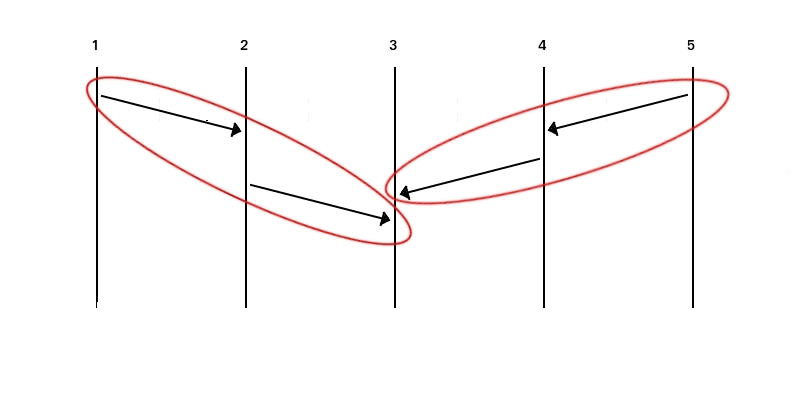
\includegraphics[width=0.5\textwidth]{fig/cut-total-ordering-partial}
  \caption{distributed program points in totally ordered subsets}
\end{figure}

%%\sc{TODO: define consistency lattice of vector clocks. talk about how all logs must be in the lattice, but the lattice itself merely gives a bound on the communication possible in the system. prove these properties with notes - prove the send/receive checksum.}

\begin{definition}[Consistent Distributed State]
    \label{def:consistent_distributed_state}Let $p_{\sigma}$, be the set of
    host states in a distributed program point $p$. Where $S$ is a
    consistent cut,  we say $\Sigma$ is consistent if.
    $\forall p, \in S, p_{\sigma} \subseteq \Sigma$.
\end{definition}



%%%%%%%%%%%%%%%%%%%%%%%%%%%%%%%%%%%%%%%%
%\begin{figure*}[t]
%    \center{\includegraphics[width=\textwidth]{fig/fig.pdf}}
%    \caption{\textbf{(a)} Five system traces (S1-S5) for a web
%        application that sells airplane tickets. Each trace consists
%        of log lines and corresponding vector clock timestamps. In the
%        traces, two clients access a single server. \textbf{(b)} A
%visualization of the five system traces as space time diagrams. Time
%flows down, and events at each host are shown in a single
%column.\label{fig:label}} \end{figure*}
%%%%%%%%%%%%%%%%%%%%%%%%%%%%%%%%%%%%%%%%

%%%%%%%%%%%%%%%%%%%%%%%%%%%%%%%%%%%%%%%%%%%%
\section{Ordering events with vector time}
\label{sec:formal-vector-clocks}
%%%%%%%%%%%%%%%%%%%%%%%%%%%%%%%%%%%%%%%%%%%%

%% We now explain the algorithm using which the
%% vector timestamps are maintained. This explanation corresponds to a
%% system that uses message passing, though vector timestamps can be used
%% for ordering event instances in a system that uses other mechanisms
%% for inter-host communication, such as shared memory.

Vector time~\cite{fidge_vector_clocks_1988,
  mattern_vector_clocks_1989} is a logical clock mechanism that
provides a partial ordering of event instances. In a distributed
system of $h$ hosts, each host maintains an array of clocks $C = [c_0,
  c_1, \dots, c_{h-1}]$, in which a clock value $c_j$ records the
local host's knowledge of (equivalently, dependence on) the local
logical time at host $j$. We denote a timestamp's $C$ clock value for
host $j$ as $C[j]$.

The hosts update their clocks to reflect the actual ordering of event
instances in the system with the following three rules:

\begin{enumerate}

    \item All hosts start with an initial vector clock value of
        $[0,\dots,0]$.

    \item When a host $i$ generates an event instance, it increments
        its own clock value (at index $i$) by 1, i.e $C_i[i]++$.

    \item When a host $h$ communicates with a host $h'$, $h$ shares
        it's current clock $C_h$ with $h'$, and $h'$ updates its local
        clock $C_{h'}$ so that $\forall i, C_{h'}[i] =
        \max\{C_h[i],C_{h'}[i]\}$. The host $h'$ also updates its local
        clock value as in (2), since message receipt is considered an
        event.

\end{enumerate}




%%%%%%%%%%%%%%%%%%%%%
\section{Logging node state}
\label{sec:logging-variables}
%%%%%%%%%%%%%%%%%%%%%

A program slice, is a subset of statements in a program, which either
affect or are affected by some root statement. Forward slicing
computes the set of statements affected by the root. Backwards slicing
computes the set of statements which affect the root. \dinv extends
Ottenstein's algorithm~\cite{Ottenstein:1984} for building a program
dependence graph (PDG) with interprocedural analysis and builds a
system dependence graph~\cite{Walkinshaw03thejava}. The roots of the
slices in Dinv are network function calls. Dinv generates the set of
variables to log by computing backwards slices from network writes and
forward slices from network reads. The general algorithm for source
code instrumentation is described in Algorithm~\ref{alg:instrument}.

Logging \emph{network interacting variables} after each executed
instruction would still produce an unmanageably large log. Dinv
resolves this by logging at just select program points. Dinv includes
two methods for identifying logging locations: a general-purpose
automated approach and an approach based on developed-supplied
annotations (Table~\ref{table:inst-strat}).

Automated dump statement injection follows a general heuristic. The
source code of the program is scanned, and annotations are injected at
the entry and exit point of each function in the program.
%
Semi-automated logging statements require the addition of annotations
by either a developer, or by automated injection. Once a program has
been annotated, \dinv analyzes the source code using program slicing,
and replaces the annotations with logging code.
Algorithm~\ref{alg:instrument} details this process at a high level.
%
Manual logging statements are specified explicitly by developers. They
specify a list of variables as arguments, and log them. This offers
fine-grained control over the instrumentation. In cases where many
variables are in scope and interact with the network the majority of
detected invariants are irrelevant to a desired system property and
obfuscate \dinv's output. We preferable when verifying invariants on
small sets of variables.

%%%%%%%%%%%%%%%%%%%%%%%%%%%%%%%%%%%%%%%%%%
\subsection{Logging functions}
\label{sec:logging-functions}
%%%%%%%%%%%%%%%%%%%%%%%%%%%%%%%%%%%%%%%%%%

One factor which complicates logging variables is their scope.
Conventionally variables are logged at a specific point in a programs
execution, this has the advantage of capturing values at a specific
moment in time, but also isolates them from being analyzed with
variables which are present in another scope. To address situations
where the variables should be logged at a specific point, and
situations where sets of variables in different scopes should be
logged together, \dinv has two distinct logging functions.

\textit{Dump} writes the values of variables directly to a log when it
is executed. Each unique dump statement is later merged as an
independent entity, the result is invariants which reflect system
invariants at arbitrary points. %Writes variables immediately to a log.

\textit{Track} writes variables to a key-value store and delays writing these
to a log until the local vector time is incremented. By deferring and
aggregating state a more complete view of a node's state can be
analyzed together, at the cost of precision.

%% The annotations for both functions are \textit{//@dump} and
%% \textit{//@track} respectively.

%%%%%%%%%%%%%%%%%%%%%%%%%%%%%%%%%%%%%%%%%%%%%%%%%%%%%%%%%%%%%%%%%
\begin{algorithm}[t]
    \KwData{Source code with dump statements $S$}
\KwResult{Instrumented Source Code $I$}

    $I$ = $S$ \\
    $dumpNode$ = CollectDumpAnnotationASTNodes($S$) \\
    \For{$dump \in dumpNodes$} {
        $variables$ = ComputeAffected($dump.line$,$S$)\\
        $loggingCode$ = NewLoggingCode($variables$, $dump.line$, $S$)\\
        $I$ += $loggingCode$\\
    }
    \Return{$Delta$}
    \caption{Algorithm converting commented logging annotation to logging code.}
    \label{alg:instrument}
\end{algorithm}
%%%%%%%%%%%%%%%%%%%%%%%%%%%%%%%%%%%%%%%%%%%%%%%%%%%%%%%%%%%%%%%%%



%%%%%%%%%%%%%%%%%%%%%%%%%%%%%%%%%%%%%%%%
\section{Constructing the lattice}
\label{sec:lattice-appendix}
%%%%%%%%%%%%%%%%%%%%%%%%%%%%%%%%%%%%%%%%

Algorithm~\ref{alg:lattice} presents the lattice construction
algorithm. Each level of the lattice is constructed sequentially.  All
clocks from the previous level have their values incremented by 1 for
each node. If the incremented clock value is valid under the
happens-before relation, it is appended to the next level of the
lattice.

%%%%%%%%%%%%%%%%%%%%%%%%%%%%%%%%%%%%%%%%%%%%%%%%%%%%%%%%%%%%%%%%%%%%%%%%%%%%%
\begin{algorithm}[t]

    \KwData{Set of Host traces $T$}
    \KwResult{Lattice representation of a System Trace $S$}
    i = 0 \;
    Level[i].append(ZeroClock())\;
    \While{!Level[i].empty()} {
        i++\;
        \For{Clock $\in$ Level[i-1]} {
            \For{Host $\in$ T}{
                Clock.increment(Host)\;
                \If {ValidLatticePoint(T,Clock)}{
                    Level[i].append(Clock)
                }
            }
        }
        $S$.append(Level[i])
    }
    \vspace{2mm}
    \caption{Lattice Construction Algorithm}
    \label{alg:lattice}
\end{algorithm}
%%%%%%%%%%%%%%%%%%%%%%%%%%%%%%%%%%%%%%%%%%%%%%%%%%%%%%%%%%%%%%%%%%%%%%%%%%%%%



%%%%%%%%%%%%%%%%%%%%%%%%%%%%%%%%%%%%%%%%%%%%%%%%%%%%%%%%
\section{Constructing strongly consistent cuts}
\label{sec:consistent-cuts-appendix}
%%%%%%%%%%%%%%%%%%%%%%%%%%%%%%%%%%%%%%%%%%%%

\textbf{Enumerating Messages}: A cut is consistent if and only if all
messages sent by nodes in a cut, were also received by a node in the
cut.  The lattice constructed in the previous section contains the set
of all possible cuts, some of which are inconsistent. If a cut is
consistent the number of in flight messages at the corresponding
vector time is zero. Checking this property can be done by iterating
through the execution logs, and counting sending and receiving events.
Because the lattice maintains the happens-before relation, If the
number of sent and received messages are equal, a cut at that time is
consistent.  Algorithm~\ref{alg:enumerate} counts the number of send
and receive events on each node by maintaining a delta of sent and
received messages.

%%%%%%%%%%%%%%%%%%%%%%%%%%%%%%%%%%%%%%%%%%%%
\begin{algorithm}[t]
    \KwData{Set of Host traces $T$}
    \KwResult{Enumerated index of Send and Receive Events $Delta$}
    \For{node $\in$ $T$} {
        \For{event $\in$ node} {
            \If{(event.WasASend())} {
                receiver, receiverEvent := logs.FindReceive(event)
                $Delta$[node][event]++
                $Delta$[receiver][receiverEvent]-\,-
            }
        }
    }
    \Return{$Delta$}
    \caption{Sent and Received message enumeration}
    \label{alg:enumerate}
\end{algorithm}
%%%%%%%%%%%%%%%%%%%%%%%%%%%%%%%%%%%%%%%%%%%


\textbf{Extracting Cuts}: The next step in the log merging process it
to process the lattice by removing all points which do not correspond
to consistent cuts.  This is done by counting all sent and received
messages at a system at each node in the lattice.  The +1 per for a
send, and -1 per a receive are stored as a \emph{delta} calculated in
the previous process. 
%
Figures~\ref{fig:time-lattice}A shows enumerated send and receive
values in red, and Figures~\ref{fig:time-lattice}B highlights the
corresponding points of the lattice which represent consistent cuts.
if the sum of the \emph{delta} for each node in a cut within the
lattice is $0$ the cut is consistent. This calculation run on each
point in the lattice produces the complete set of consistent cuts.  An
abstract version of this process can be found in
Algorithm~\ref{alg:mineCuts}.

%\begin{figure}[h]
%    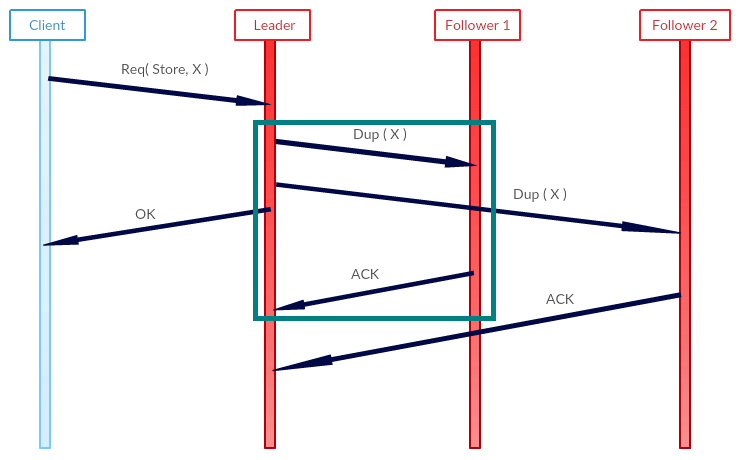
\includegraphics[width=0.5\textwidth]{fig/highlighted-lattice}
%  \caption{Subset of example execution}
%\end{figure}

\begin{algorithm}
 \KwData{$lattice$, $clocks$, $delta$}
 \KwResult{$cuts$}
 \For{$level \in lattice$} {
    \For{$node \in level$} {
        $delta$ := $0$;
        \If{$node \in clocks$} {
            \For{$node$,$clockValue$ $\in$ $node$} {
                $delta$ += $deltaComm$[$node$][$clockValue$]
            }
       }
       \If{$delta$ == $0$} {
            $cuts$.append($node$)
       }
    }
 }
 \Return{$cuts$}

    \vspace{2mm}
 \caption{Algorithm for determining which lattice points correspond to a consistent cut}
 \label{alg:mineCuts}
\end{algorithm}



%%%%%%%%%%%%%%%%%%%%%%%%%%%%%%%%%%%%%%%%%%%%
\textbf{Collecting Hosts States}: Next we collect the set of node
states  at the logical times they occurred in each consistent cut.
This computation is done by searching the execution logs for node
states with matching vector clock values.
%
One challenge is the lack of a one-to-one correspondence between node
states, and vector clock values.  This is the consequence of either
having \textit{Dump} statements log a nodes state multiple times
before incrementing its clock value, or having no dump statement
executed at the given time. In such situations we choose the logged
state based on the last networking operation performed by the node. In
the case where the last operation was a receive, the node state
corresponding to the earliest event instance is selected. Conversely
if the last operation was to send a message, the node state
corresponding to the last event instance is selected.  If no node
state is available it is not merged. In
Section~\ref{sec:logging-functions} we introduced \textit{Track}
logging functions to mitigate this complication.  \textit{Track} which
logs variables to a key value store, and only writes to a log during
increments of vector time.  Logging with a key value store has the
advantage of aggregating node state and providing a one to one
correspondence between vector time and and logged state, but has the
disadvantage of missing multiple intermediate state transitions during
a single vector time.  The output of this process is the complete set
of node states at every point during execution when all state was
resident in memory. 

\begin{figure}[h]
    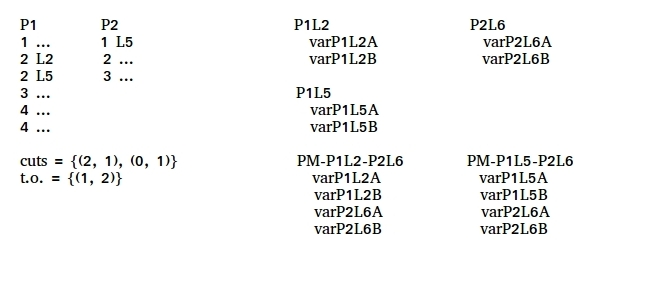
\includegraphics[width=0.5\textwidth]{fig/merge-point-logs}
  \caption{Retrieve consistent node states from logs}
\end{figure}

%%%%%%%%%%%%%%%%%%%%%%%%%%%%
\begin{algorithm}
 \KwData{$Cuts$, $Log$}
 \KwResult{Set of consistent node states $S$}
 \For{$Cut \in Cuts$} {
     \For{$Host$,$Clock \in Cut$} {
         $s$ += getHostStateFromLog($Host$,$Clock$,$Log$)
     }
     $S$.append($s$)
 }
 \Return{$S$}

 \caption{Collect the Host's state, for each consistent cut}
 \label{alg:collectStates}
\end{algorithm}
%%%%%%%%%%%%%%%%%%%%%%%%%%%%



%%%%%%%%%%%%%%%%%%%%%%%%%%%%%%%%%%%%%%%%%%%
\section{Daikon background}
\label{daikon-appendix}
%%%%%%%%%%%%%%%%%%%%%%%%%%%%%%%%%%%%%%%%%%%

Daikon is a dynamic analysis tool which automatically detects likely
data invariants in sequential systems. Daikon derives data invariants
by processing data traces (\emph{dtraces}) produced during the run
time of a program. A trace consists of a set of variable names, and
the various values they took over the course of a programs
execution. To produce a system trace Daikon injects logging statements
at the beginning and end of both functions and loops, which dump the
values of all variables in scope. Daikon uses a confidence measure to
filter our spurious invariants.

\begin{lstlisting}[
    caption={simple program with loop invariants},
    label={lst:loopinvariants}
    ]
i := 0
j := 1
k := i + j
for i < 5 {
    k = i + j
    i++
    j++
}
\end{lstlisting}

\begin{lstlisting}[
    caption={Code instrumented to produce trace},
    label={lst:insturmenteddaikonLoop}
    ]
i := 0
j := 1
k := i + j
for i < 5 {
    logToTrace(i,j,k)
    k = i + j
    i++
    j++
    logToTrace(i,j,k)
}
\end{lstlisting}

\begin{table}
        \caption{Daikon Invariants}
        \label{table:daikon-invariants}
    \begin{framed}
        \begin{enumerate}[noitemsep]
                \item $k = i + j$
                \item $j > i$
                \item $j = i + 1$
                \item $i < 5$
        \end{enumerate}
   \end{framed}
\end{table}

%%%%%%%%%%%%%%%%%%%%%%%%%%%%%%%%%%%%%%%%%%%
\subsection{Translation Daikon invariants to first order logic}
\label{sec:daikon-to-fol}
%%%%%%%%%%%%%%%%%%%%%%%%%%%%%%%%%%%%%%%%%%%

Daikon supports unary, binary, and ternary invariants out of the box,
and does not support predicate logic.  The result of this is that
invariant properties that hold over sets of $n$ variables are output
in pieces. For example if 4 variables $X_0 \dots X_3$ were determined
to always be equal Daikon's output would appear as $X_0 == X_1$, $X_0
== X_2$, $X_0 == X_3$. In this case the 4 invariants can be combined
transitively to show equality among all of them. In such cases we
present the invariant as a first order logical formula. For example in
this case the invariant would be denoted $\forall i,j$, $X_i = X_j$.

In other cases an invariant property is that in a single case a
property exists. As an example in Section~\ref{sec:application} we
espouse the strong leadership principle of raft, stating that only a
leader is able to issue an append entries message, and should
therefore have a log greater than or equal to each of the followers.
In this case we logged host state in two separate functions, one for
followers, and one for the leader. The Daikon output from the
execution was a separate file for each host which was a leader during
execution. Detailed in Table~\ref{table:Existance-Invariant} is the
set of invariants used to support the property of strong leadership in
etcd raft. The table supposes a cluster was composed of 3 hosts
$A$,$B$,$C$ each of which became a leader at least once. From the
output it can be inferred that If a host is in the state leader, it
has a log larger than that of the followers, and the followers have
logs of equal size. For conciseness we represent this invariant with the following formula $Leader-LogSize >= Followers-LogSize $,$\forall followers$.

\begin{table}
        \caption{Raft Strong Leadership Invariant}
        \label{table:Existance-Invariant}
    \begin{framed}
        \caption{File A-Leader B-Follower C-Follower}
        \begin{enumerate}[noitemsep]
                \item $A-State == Leader$
                \item $C-State == B-State$
                \item $B-State == Follower$
                \item $A-LogSize >= B-LogSize$
                \item $A-LogSize >= C-LogSize$
                \item $B-LogSize == C-LogSize$
        \end{enumerate}
        \caption{File A-Follower B-Leader C-Follower}
        \begin{enumerate}[noitemsep]
                \item $B-State == Leader$
                \item $A-State == C-State$
                \item $A-State == Follower$
                \item $B-LogSize >= A-LogSize$
                \item $B-LogSize >= C-LogSize$
                \item $A-LogSize == C-LogSize$
        \end{enumerate}
        \caption{File A-Follower B-Follower C-Leader}
        \begin{enumerate}[noitemsep]
                \item $C-State == Leader$
                \item $A-State == B-State$
                \item $B-State == Follower$
                \item $C-LogSize >= B-LogSize$
                \item $C-LogSize >= A-LogSize$
                \item $B-LogSize == A-LogSize$
        \end{enumerate}
   \end{framed}
\end{table}



\balance
\bibliographystyle{abbrv}
\bibliography{paper}

\end{document}
